\documentclass[11pt,letterpaper]{article}
\usepackage[margin=1in,headheight=15pt]{geometry}
\usepackage[T1]{fontenc}
\usepackage{newpxtext}
\usepackage{amsmath,amsthm,mathtools}
\usepackage{newpxmath}
\usepackage{microtype}
\usepackage[table]{xcolor}
\usepackage{booktabs,tabularx,array,longtable}
\usepackage{enumitem}
\usepackage{tikz}
\usetikzlibrary{positioning,arrows.meta}
\usepackage[most]{tcolorbox}
\usepackage{listings}
\usepackage{fancyhdr}
\usepackage{titlesec}
\usepackage{hyperref}
\usepackage{bookmark}
\definecolor{forest}{HTML}{264B3D}
\definecolor{olive}{HTML}{737A43}
\definecolor{sage}{HTML}{EDF2EC}
\definecolor{ink}{HTML}{23312C}
\definecolor{muted}{HTML}{5C6860}
\hypersetup{colorlinks=true,linkcolor=forest,citecolor=forest,urlcolor=forest,
 pdftitle={Friendly Order Types of Finite Posets and Ordinal Products},
 pdfauthor={ChatGPT, research report prepared for Vladimir Reshetnikov},
 pdfsubject={Exact formulas and a compositionality obstruction for the friendly order type},
 pdfkeywords={well-partial-order, friendly order type, ordinal product, natural product, incomparability graph}}
\titleformat{\section}{\Large\bfseries\color{forest}}{\thesection}{0.7em}{}
\titleformat{\subsection}{\large\bfseries\color{forest}}{\thesubsection}{0.7em}{}
\titleformat{\subsubsection}{\normalsize\bfseries\color{forest}}{\thesubsubsection}{0.7em}{}
\titlespacing*{\section}{0pt}{2.5ex plus 1ex minus .2ex}{1.1ex}
\titlespacing*{\subsection}{0pt}{1.8ex plus .8ex minus .2ex}{.7ex}
\pagestyle{fancy}
\fancyhf{}
\fancyhead[L]{\small\color{muted}\textsc{Friendly order types}}
\fancyhead[R]{\small\color{muted}Research report / 19 September 2026}
\fancyfoot[C]{\color{forest}\thepage}
\renewcommand{\headrulewidth}{0.3pt}
\renewcommand{\footrulewidth}{0pt}
\setlength{\parskip}{.35em}
\setlength{\parindent}{1.1em}
\setcounter{tocdepth}{1}
\setlist{itemsep=.25em,topsep=.4em}
\newtheorem{theorem}{Theorem}[section]
\newtheorem{lemma}[theorem]{Lemma}
\newtheorem{proposition}[theorem]{Proposition}
\newtheorem{corollary}[theorem]{Corollary}
\theoremstyle{definition}
\newtheorem{definition}[theorem]{Definition}
\newtheorem{example}[theorem]{Example}
\newtheorem{question}[theorem]{Question}
\theoremstyle{remark}
\newtheorem{remark}[theorem]{Remark}
\newcommand{\fot}{f}
\newcommand{\mot}{o}
\newcommand{\str}{\operatorname{str}}
\newcommand{\pred}{\operatorname{pred}}
\newcommand{\Bad}{\operatorname{Bad}}
\newcommand{\Fr}{\operatorname{Fr}}
\newcommand{\Inc}{\operatorname{Inc}}
\newcommand{\res}[2]{#1_{\not\ge #2}}
\newcommand{\N}{\mathbb{N}}
\newcommand{\epsmin}{\varepsilon_{\min}}
\newcommand{\epsmax}{\varepsilon_{\max}}
\newcommand{\wpo}{\textnormal{wpo}}
\newcommand{\one}{\mathbf{1}}
\newcommand{\chain}[1]{\mathbf{#1}}
\newcommand{\anti}[1]{\Gamma_{#1}}
\newtcolorbox{resultbox}[1][]{colback=sage,colframe=forest,boxrule=.5pt,
 arc=1.5mm,left=3mm,right=3mm,top=2mm,bottom=2mm,breakable,#1}
\lstset{basicstyle=\small\ttfamily,columns=fullflexible,keepspaces=true,
 breaklines=true,frame=single,rulecolor=\color{olive},backgroundcolor=\color{sage},
 showstringspaces=false,aboveskip=.8em,belowskip=.8em}
\newcolumntype{Y}{>{\raggedright\arraybackslash}X}
\begin{document}
\begin{titlepage}
\color{ink}
\vspace*{.03in}
{\small\bfseries\color{olive}\MakeUppercase{Order theory \enspace / \enspace Ordinal combinatorics}}
\par\vspace{.2in}
{\fontsize{29}{33}\selectfont\bfseries\color{forest}Friendly Order Types\par}
\vspace{.08in}
{\fontsize{27}{31}\selectfont\bfseries\color{forest}of Finite Posets and\par Ordinal Products\par}
\vspace{.18in}
{\large Exact formulas, a compositionality obstruction,\par and a finite-tail method\par}
\vspace{.18in}
\noindent\textcolor{olive}{\rule{\textwidth}{1pt}}
\vspace{.16in}
\noindent\textbf{Research report}\hfill 19 September 2026\\[.35em]
Prepared for Vladimir Reshetnikov \hfill Prepared by ChatGPT
\vspace{.14in}
\begin{resultbox}[title={\bfseries Main conclusions}]
\small
For a finite poset $P$, let $c(P)$ count the connected components of its
incomparability graph, including isolated vertices. Then
\[
 \fot(P)=|P|-c(P).
\]
For a non-chain finite Cartesian product of ordinals, the infinite case has
friendly order type equal to its natural product, except that one rightmost
successor is removed when every factor is a successor ordinal. The result
extends to products of infinite ordinals with an arbitrary finite poset.

Two four-element posets with identical $(o,h,w,f)$ give different friendly
order types after multiplication by the same two-element chain. Thus those
four numerical invariants do not support a general product formula.
\end{resultbox}
\vspace{.14in}
\small
\noindent\textbf{Abstract.}
The compositional calculation of friendly order type is an explicitly
identified research direction in work of Isa Vialard. We study finite
posets, products, and finite successor tails of ordinal products. Our
finite formula follows from a deletion lemma for connected incomparability
graphs. A projection argument shows that a nontrivial Cartesian product
has a single non-endpoint incomparability component. We then isolate the
finite upper corner of an infinite ordinal product and construct legal
friendly deletions of that corner. This gives exact transfinite formulas,
not merely finite approximations. The accompanying software independently
checks the finite formula, verifies a small compositionality counterexample,
and implements hereditary Cantor normal forms below $\varepsilon_0$.

\vfill
\noindent{\small\color{muted}\textbf{Status.} Conventional proofs are supplied for the results developed here.
The transfinite argument uses explicitly cited published theorems.
This is a research draft, not a peer-reviewed or formally verified paper.
No publication-priority claim is made.}
\end{titlepage}

\tableofcontents
\vspace{1em}
\begin{resultbox}[title={\bfseries Reading guide}]
Sections~\ref{sec:finite}--\ref{sec:counterexample} are finite and elementary.
Sections~\ref{sec:tails}--\ref{sec:mixed} contain the transfinite argument.
The complete classification of ordinal boxes is in
Theorem~\ref{thm:boxes}. Section~\ref{sec:computation} and the appendices
explain exactly what the software verifies and what it does not verify.
\end{resultbox}
\clearpage

\section{The selected problem and its scope}\label{sec:scope}

\subsection{A documented open direction}
Vialard introduced the friendly order type $o_\perp(P)$ in the study of
ordinal widths of finite multiset orderings. The conclusion of the MFCS
2023 paper asks about further compositional calculations of this invariant
\cite[Conclusion, p.~87:11]{Vialard2023}. The conclusion of the subsequent
thesis again presents its compositional computation as a research direction
\cite[Conclusion, p.~109]{VialardThesis}. We write $f(P)$ instead of
$o_\perp(P)$ throughout this report.

The broad question needs a precise interpretation. A construction may be
computable from a rich structural description of its inputs without being
a function of a short list of their ordinal invariants. These are different
notions of compositionality. We investigate both, through the following
restricted questions.

\begin{question}\label{q:finite}
Can the friendly order type of an arbitrary finite poset be recovered
from a simple structural statistic, without constructing its entire
friendly bad-sequence tree?
\end{question}

\begin{question}\label{q:scalar}
Is $f(A\times B)$ determined by the two tuples
\[
 (o(A),h(A),w(A),f(A))\quad\text{and}\quad(o(B),h(B),w(B),f(B))?
\]
\end{question}

\begin{question}\label{q:ordinal}
Can one compute $f(P)$ exactly when $P$ is a finite product of ordinals,
or more generally a product of infinite ordinals with a finite poset?
\end{question}

These precise questions are formulations adopted in this report; we do
not attribute them verbatim to Vialard. We answer the first and third
positively and the second negatively. This resolves specified subproblems
of the published program, not the unrestricted program for arbitrary
well-partial-orders and arbitrary constructions.

\subsection{What was already known}
The limit-ordinal case must not be mistaken for a new result. Vialard's
thesis already proves
\[
 f(A\times B)=o(A\times B)
 \quad\text{if both $o(A)$ and $o(B)$ are limit ordinals}
\]
\cite[Theorem~5.4.8(3)]{VialardThesis}.
The binary ordinal-sum rule is also known. We use these facts for context,
not as claims of novelty. Our transfinite proof rests on the published
limit-saturation theorem stated in Section~\ref{sec:preliminaries}; the
additional work is to control stripping and the finite successor corner
exactly.

\subsection{What this report establishes}
Theorem~\ref{thm:finite} gives the finite formula $f(P)=|P|-c(P)$.
Theorem~\ref{thm:product-components} identifies the incomparability
components of every Cartesian product with two non-singleton factors.
Theorem~\ref{thm:no-scalar} gives an explicit counterexample to
Question~\ref{q:scalar}. Theorem~\ref{thm:mixed} settles the mixed
ordinal--finite product problem, including the distinction between a
finite factor with and without a greatest element.

A useful feature is that the strongest theorem is not restricted to
countable ordinals. The proofs take place in ZFC and apply to arbitrary
set-sized ordinals. The executable ordinal notation system is deliberately
more restricted: it handles ordinals below $\varepsilon_0$, which admit
finite hereditary Cantor normal forms.

\subsection{Literature and novelty status}
The source check for this report was made on 19 September 2026. It included
the official MFCS proceedings version, the author-hosted thesis, the
author's publication list, and searches for the invariant under its
published and earlier terminology. The prepublication arXiv version uses
``maximal safe order type''; definitions and citations here follow the
published friendly-order-type treatment.

The exact finite formula, the particular obstruction, and the complete
successor-tail calculation below were not located in the sources checked.
That is a limited literature-search conclusion, not a proof of priority.
The appropriate status is: \emph{results proved in this draft, with
independent expert review and a fuller novelty check still desirable}.
The argument is not presented as a resolution of an unrelated famous
conjecture, nor is computational agreement presented as a transfinite
proof.

\section{Definitions and proof dependencies}\label{sec:preliminaries}

\subsection{Well-partial-orders and residuals}
A finite or infinite sequence $x_0,x_1,\ldots$ in a poset $P$ is
\emph{bad} if there is no pair $i<j$ with $x_i\le x_j$. A
\emph{well-partial-order}, abbreviated wpo, has no infinite bad sequence.
For $x\in P$, write
\[
 \uparrow x=\{y\in P:x\le y\},\qquad
 \res P x=P\setminus\uparrow x.
\]
For a finite sequence $s$, the residual is
\[
 \res P s=P\setminus\bigcup_{x\text{ occurring in }s}\uparrow x.
\]
Every next term of a bad sequence belongs to the current residual.
All orders on subsets in this report are induced orders.

A well-founded tree has rank given recursively by
\[
 \operatorname{rk}(s)
 =\sup\{\operatorname{rk}(s^{\frown}x)+1:s^{\frown}x\text{ is in the tree}\},
\]
where the supremum of the empty set is zero. The tree rank is the rank of
the empty sequence. It need not be the supremum of the finite lengths of
its branches. This distinction will be essential.

\subsection{The friendly restriction}
Two points are \emph{incomparable}, written $x\perp y$, when neither is
below the other. A bad sequence is \emph{friendly} (called open-ended in
the original definition) if, when each term $x$ is selected, the current
residual contains a point $y\perp x$. The point $y$ is a friend witnessing
that move. This is the definition from
\cite[Definition~5.3.2]{VialardThesis}.

The empty sequence is friendly. A friend need not be selected later.
Because it is incomparable with $x$, it survives the deletion of
$\uparrow x$. Let $\Fr(P)$ be the tree of friendly bad sequences, and
let $f(P)$ be its rank. Equivalently,
\begin{equation}\label{eq:f-residual}
 f(P)=\sup_{\substack{x\in P\\ \exists y\in P\ (x\perp y)}}
       \bigl(f(\res P x)+1\bigr).
\end{equation}
For a finite poset this rank is the maximum number of legal moves. For an
infinite wpo it is an ordinal rank, not an infinite play: all individual
plays remain finite.

\begin{lemma}[Basic properties]\label{lem:basic}
For wpos $S\subseteq P$, with induced order,
\[
 f(S)\le f(P),\qquad f(P)\le o(P).
\]
Also $f(P)=0$ exactly when $P$ is a chain, including the empty chain.
If a legal sequence of $k$ moves leaves residual $R$, then
\begin{equation}\label{eq:moves}
 f(P)\ge f(R)+k.
\end{equation}
The addition in this formula is ordinary ordinal addition on the right.
\end{lemma}
\begin{proof}
A friendly sequence in $S$, with its friends in $S$, remains friendly in
$P$: an earlier selected point removes precisely the same points of $S$
in either ambient poset. Thus $\Fr(S)$ is a subtree of $\Fr(P)$.
The friendly tree is a subtree of the full bad-sequence tree, which gives
the second inequality. Equation~\eqref{eq:f-residual} has an eligible first
move exactly when an incomparable pair exists. Finally apply
\eqref{eq:f-residual} successively along the specified legal sequence.
Each step adds a successor on the right, so after $k$ steps the lower
bound is $f(R)+k$.
\end{proof}

\subsection{The stripped poset}
Define
\[
 \str(P)=\{x\in P:\exists y\in P\ (x\perp y)\}.
\]
It removes every point comparable with all points of $P$. Every selected
point of a friendly sequence belongs to $\str(P)$, so
\begin{equation}\label{eq:strip-upper}
 f(P)\le o(\str(P)).
\end{equation}
Notice that stripping can remove more than endpoints in a general poset.
The fact that products behave much better is one of the main structural
lemmas of this report.

\subsection{Imported theorems}
We explicitly isolate the external results used in the transfinite part.
The maximal order type $o(P)$ is the rank of the bad-sequence tree. The
maximal-linearization theorem of de Jongh and Parikh identifies it with an
\emph{attained} maximum among order types of well-order linear extensions.
For wpos $A,B$,
\begin{equation}\label{eq:mot-product}
 o(A\times B)=o(A)\otimes o(B),
\end{equation}
where $\otimes$ is the natural product \cite{DeJonghParikh}.
The use of an attained maximum, rather than just a supremum, matters in
Lemma~\ref{lem:upper-tail}.

\begin{theorem}[Published limit saturation]\label{thm:imported-limit}
If $P$ is a wpo, $o(P)$ is a nonzero limit ordinal, and
$o(\str(P))=o(P)$, then
\[
 f(P)=o(P).
\]
\end{theorem}
This is Vialard's Corollary~4.7 \cite{Vialard2023}. Its proof is not
reproduced here. Accordingly, our transfinite proofs are complete
\emph{relative to this explicitly stated published theorem}, not a new
self-contained derivation of the entire underlying theory.

A second imported result supplies a useful application. Let $M^r(P)$ be
the set of finite multisets with the multiset ordering: $m<_r n$ when
$m\ne n$ and every occurrence left in $m\setminus n$ is strictly below
some occurrence in $n\setminus m$. Differences here cancel common
multiplicities; the domination need not be injective. Vialard proves
\begin{equation}\label{eq:multiset}
 w(M^r(P))=\omega^{f(P)}
\end{equation}
\cite[Theorem~3.4]{Vialard2023}. This is \emph{not} the distinct multiset
embedding order. We use \eqref{eq:multiset} only for consequences, not for
any main proof.

The ordinal height and width are the ranks of the trees of strictly
decreasing sequences and antichains, respectively. For finite posets they
are the ordinary largest chain and antichain cardinalities. For infinite
wpos, ordinal width is not simply the supremum of finite antichain sizes.

\section{Every finite poset: a component formula}\label{sec:finite}

\subsection{Incomparability components are ordered blocks}
Let $\Inc(P)$ be the undirected graph with vertex set $P$, in which two
vertices are adjacent exactly when they are incomparable. Write $c(P)$
for its number of connected components when $P$ is finite, counting
isolated vertices. Put $c(\varnothing)=0$.

\begin{lemma}[Ordered components]\label{lem:ordered-components}
Distinct connected components of $\Inc(P)$ are uniformly comparable.
They therefore form linearly ordered ordinal-sum blocks: for two distinct
components $C,D$, either every point of $C$ is below every point of $D$,
or every point of $D$ is below every point of $C$.
\end{lemma}
\begin{proof}
Points in distinct components must be comparable, since otherwise they
would be adjacent. Suppose $x\perp x'$ lie in one component and $z$ lies
in another. Opposite orientations, such as $x<z<x'$, contradict
$x\perp x'$. Thus the orientation of comparison with $z$ is constant
along every incomparability edge and hence along every path. Applying the
same argument to paths in the second component gives uniform comparison
between the two components. Transitivity and antisymmetry of $P$ make the
resulting comparison a linear order on the set of components.
\end{proof}

For a wpo the component order is itself a well-order: an infinite
descending sequence of components, with one representative from each,
would be a bad sequence. For the finite theorem we need only the elementary
finite version of this observation.

\subsection{A maximal point can be deleted without disconnecting}

\begin{lemma}[Maximal non-cut vertex]\label{lem:noncut}
If $P$ is finite, $|P|>1$, and $\Inc(P)$ is connected, then $P$ has a
maximal element $v$ such that $\Inc(P\setminus\{v\})$ is connected.
\end{lemma}
\begin{proof}
Choose a maximal element $u$. If deleting $u$ leaves a connected graph,
there is nothing to prove. Otherwise, by Lemma~\ref{lem:ordered-components},
the components of $P\setminus\{u\}$ can be written
\[
 C_1<C_2<\cdots<C_k,\qquad k\ge2.
\]
Connectivity of $\Inc(P)$ forces $u$ to have a neighbor in every $C_i$.
Choose $a\in C_1$ with $a\perp u$.

For $z\in C_j$ with $j>1$, we have $a<z$. The relation $z<u$ would imply
$a<u$, while $u<z$ contradicts maximality of $u$. Thus
\begin{equation}\label{eq:u-universal}
 u\perp z\quad\text{for every }z\in C_2\cup\cdots\cup C_k.
\end{equation}
Choose a maximal element $v$ of $C_k$. It is maximal in $P$: nothing in an
earlier component can be above it, nothing in $C_k$ is strictly above it,
and $u$ is incomparable with it.

After deleting $v$, all the earlier components remain connected internally
and attached to $u$. Every surviving vertex of $C_k$ is directly adjacent
to $u$ by \eqref{eq:u-universal}. If $C_k=\{v\}$, this last requirement is
vacuous. The remaining graph is connected in either case.
\end{proof}

The order-theoretic word ``maximal'' is important. A connected graph always
has non-cut vertices, but an arbitrary non-cut vertex need not delete
only itself under the friendly residual operation. A maximal point does:
its principal upper set within the current component is a singleton.

\begin{corollary}\label{cor:connected-finite}
For a finite nonempty poset with connected incomparability graph,
\[
 f(P)=|P|-1.
\]
\end{corollary}
\begin{proof}
Repeatedly apply Lemma~\ref{lem:noncut}. As long as at least two vertices
remain, the connected incomparability graph gives the chosen vertex a
friend. Maximality means the move removes only that vertex. The process
makes $|P|-1$ moves and leaves one point.

No friendly sequence can select every point of a nonempty finite poset:
the final selected point would require an available incomparable point
that had not already been selected. Hence $|P|-1$ is also an upper bound.
\end{proof}

\subsection{The exact formula}

\begin{theorem}[Finite friendly order type]\label{thm:finite}
For every finite poset $P$,
\begin{equation}\label{eq:finite-formula}
 \boxed{f(P)=|P|-c(P).}
\end{equation}
\end{theorem}
\begin{proof}
The empty case is immediate. Write the incomparability components as
$C_1<\cdots<C_k$.

For the upper bound, consider any friendly sequence. Within each original
component that contains a selected point, take its \emph{last selected
point} $x$. Its friend belongs to the same original component, since an
incomparability edge cannot connect distinct components. That friend was
not selected earlier, because earlier selected points are absent from the
current residual, and it is not selected later, by the choice of $x$.
Thus every component with a selected point contains a point never selected.
A component with no selected points plainly does too. At least $k$ points
of $P$ are never selected, so the sequence has length at most $|P|-k$.
This argument allows points to be removed incidentally without being
selected; it does not confuse these two events.

For the lower bound, process the components from $C_k$ down to $C_1$.
Within $C_i$, use Corollary~\ref{cor:connected-finite} to select
$|C_i|-1$ points. A move in a higher component never removes a point of
a lower component. When a lower component is processed, it may remove
unselected leftovers of higher components, but these are no longer needed.
The friends and maximal deletions inside the current component remain
valid. We obtain
\[
 \sum_{i=1}^k(|C_i|-1)=|P|-k
\]
legal moves, completing the proof.
\end{proof}

\subsection{Sharp bounds in terms of the stripped cardinality}

\begin{corollary}\label{cor:finite-strip}
Let $s=|\str(P)|$ and let $k$ be the number of non-singleton
incomparability components of a finite poset $P$. Then
\[
 f(P)=s-k.
\]
If $s=0$, then $f(P)=0$. The value $s=1$ is impossible. For every $s\ge2$,
\begin{equation}\label{eq:sharp-finite-bounds}
 \left\lceil\frac{s}{2}\right\rceil\le f(P)\le s-1,
\end{equation}
and every integer in this interval occurs.
\end{corollary}
\begin{proof}
Stripping removes exactly the isolated vertices of the incomparability
graph. Each remaining component has at least two vertices. Thus
$1\le k\le\lfloor s/2\rfloor$ when $s>0$, and the formula gives the bounds.
For any allowed $k$, partition $s$ into $k$ integers at least two and take
an ordinal sum of antichains of those sizes. Its stripped cardinality is
$s$ and its friendly order type is $s-k$. This realizes every value.
\end{proof}

For example, $f(\anti n)=n-1$ for a nonempty $n$-element antichain, while
$f(\chain n)=0$ for a chain. An ordinal sum of five two-element antichains
has ten stripped points but friendly order type five, whereas a ten-point
antichain has friendly order type nine. The arrangement into ordinal-sum
blocks, not simply the number of incomparable points, is decisive.

Combining Theorem~\ref{thm:finite} with the imported multiset identity gives
\begin{equation}\label{eq:finite-multiset}
 w(M^r(P))=\omega^{|P|-c(P)}
 \qquad(P\text{ finite}).
\end{equation}
The finite graph statistic therefore determines an infinite ordinal width.

\section{Incomparability components of products}\label{sec:products}

\subsection{A projection obstruction to nontrivial ordinal cuts}
An ordinal cut $P=L+U$ means that $L,U$ partition $P$, are nonempty, and
every element of $L$ is strictly below every element of $U$. This is much
stronger than saying that $L$ is a downset.

\begin{lemma}[Product cut lemma]\label{lem:cut}
Let $A,B$ be posets with $|A|,|B|\ge2$. If
\[
 A\times B=L+U,
\]
then either $|L|=1$ or $|U|=1$.
\end{lemma}
\begin{proof}
Write $A_L,A_U$ for the projections of $L,U$ to $A$, and $B_L,B_U$ for
the projections to $B$. Every point of $A_L$ is below every point of
$A_U$; the analogous assertion holds in $B$. Consequently each of
$A_L\cap A_U$ and $B_L\cap B_U$ contains at most one point. Indeed, two
points in such an intersection would each be below the other.

Because $A_L\cup A_U=A$ and $|A|\ge2$, some element of $A$ belongs to
exactly one of the two projections. Suppose first that
$a\in A_L\setminus A_U$. The whole fiber $\{a\}\times B$ lies in $L$,
so $B_L=B$. Every element of the nonempty set $B_U$ is then a greatest
element of $B$, so $B_U$ is a singleton. Choose
$b\in B\setminus B_U$. The whole fiber $A\times\{b\}$ lies in $L$,
so $A_L=A$. It follows similarly that $A_U$ is a singleton consisting of
a greatest element of $A$. Therefore $U\subseteq A_U\times B_U$ is a
singleton.

If instead $a\in A_U\setminus A_L$, the order-dual argument makes $L$
a singleton. No finiteness or well-foundedness assumption was used.
\end{proof}

\begin{theorem}[One non-endpoint component]\label{thm:product-components}
Let $A,B$ be posets with $|A|,|B|\ge2$. The incomparability components of
$A\times B$ are exactly:
\begin{enumerate}[label=(\roman*)]
\item a singleton least element, when both factors have least elements;
\item one connected component containing every non-endpoint point;
\item a singleton greatest element, when both factors have greatest elements.
\end{enumerate}
The middle component is nonempty and has at least two points. Missing
endpoints are simply omitted from this description.
\end{theorem}
\begin{proof}
By Lemma~\ref{lem:ordered-components}, the components are linearly ordered.
There cannot be four distinct components: choose four in increasing order
and cut after the second of these, including all components below it.
Both sides then contain at least two points, contradicting
Lemma~\ref{lem:cut}.

If there are three components, cutting after the first forces the first
to be a singleton, and cutting before the last forces the last to be a
singleton. Since $|A\times B|\ge4$, the middle has at least two points.
If there are two components, the cut lemma says one is a singleton;
the other has at least three points. If there is one component, it contains
at least four points. Thus precisely one component is non-singleton, and
any other components are endpoint singletons.

A singleton first component is a least element of the product; a singleton
last component is a greatest element. Conversely, a least or greatest
point is comparable with every point and hence is an isolated vertex of
the incomparability graph. Finally a product has a least element exactly
when both factors do, and the same equivalence holds for greatest
elements. This proves all assertions.
\end{proof}

The theorem applies to an arbitrary finite product with at least two
non-singleton factors: group one non-singleton factor against the product
of the others. Singleton factors can be removed without changing the
poset.

\subsection{Exact finite product formula}

\begin{corollary}\label{cor:finite-product}
Let $A,B$ be finite posets of cardinality at least two. Put
\[
 \epsmin=\begin{cases}1&\text{both have least elements},\\0&\text{otherwise},\end{cases}
 \qquad
 \epsmax=\begin{cases}1&\text{both have greatest elements},\\0&\text{otherwise}.\end{cases}
\]
Then
\begin{equation}\label{eq:finite-product}
 \boxed{f(A\times B)=|A||B|-1-\epsmin-\epsmax.}
\end{equation}
For at least two non-singleton finite factors, the same formula holds
with the product cardinality and the all-factors endpoint flags.
\end{corollary}
\begin{proof}
The number of incomparability components is
$1+\epsmin+\epsmax$ by Theorem~\ref{thm:product-components}. Apply
Theorem~\ref{thm:finite}.
\end{proof}

This is a genuine compositional formula after enriching the input data by
two Boolean endpoint flags. The next section shows why some such additional
information is necessary: it is not recoverable from the four numerical
invariants in Question~\ref{q:scalar}.

\section{A finite obstruction to scalar compositionality}\label{sec:counterexample}

\subsection{Two four-element factors}
Let
\[
 D=\one+\anti2+\one,
 \qquad
 E=\anti2+\one+\one,
 \qquad K=\chain2.
\]
Write the elements of $D$ as $a_0,a_1,a_2,a_3$, with $a_0$ least,
$a_1\perp a_2$, and $a_3$ greatest. In $E$, the points $b_0,b_1$ are
incomparable minima, both below $b_2<b_3$.

\begin{figure}[ht]
\centering
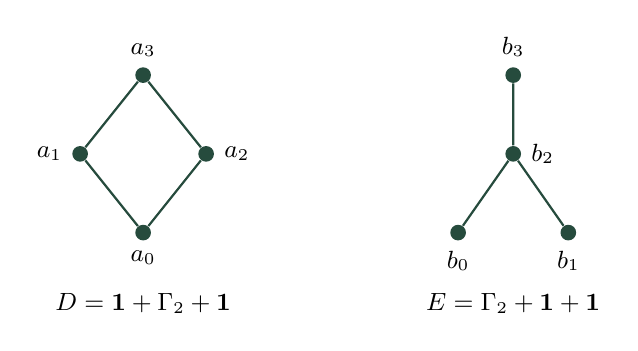
\begin{tikzpicture}[every node/.style={font=\small},
 dot/.style={circle,fill=forest,inner sep=2pt}]
 \node[dot,label=below:$a_0$] (a0) at (0,0) {};
 \node[dot,label=left:$a_1$] (a1) at (-.8,1) {};
 \node[dot,label=right:$a_2$] (a2) at (.8,1) {};
 \node[dot,label=above:$a_3$] (a3) at (0,2) {};
 \draw[forest,thick] (a0)--(a1)--(a3)--(a2)--(a0);
 \node at (0,-.9) {$D=\one+\anti2+\one$};
 \node[dot,label=below:$b_0$] (b0) at (4,0) {};
 \node[dot,label=below:$b_1$] (b1) at (5.4,0) {};
 \node[dot,label=right:$b_2$] (b2) at (4.7,1) {};
 \node[dot,label=above:$b_3$] (b3) at (4.7,2) {};
 \draw[forest,thick] (b0)--(b2)--(b1) (b2)--(b3);
 \node at (4.7,-.9) {$E=\anti2+\one+\one$};
\end{tikzpicture}
\caption{Hasse diagrams of the two factors. They have the same four
numerical invariants but different least-element flags.}
\label{fig:counterexample}
\end{figure}

Both have four points, height three, width two, and three incomparability
components. Consequently
\begin{equation}\label{eq:factor-tuples}
 (o(D),h(D),w(D),f(D))=(o(E),h(E),w(E),f(E))=(4,3,2,1).
\end{equation}
The factor $D$ has both endpoints. The factor $E$ has a greatest element
but no least element. Corollary~\ref{cor:finite-product} gives
\begin{equation}\label{eq:counterexample-values}
 f(D\times K)=8-3=5,
 \qquad
 f(E\times K)=8-2=6.
\end{equation}

\begin{theorem}[No formula from the four factor invariants]\label{thm:no-scalar}
There is no function $\Phi$ of eight ordinal arguments such that, for all
wpos $A,B$,
\[
 f(A\times B)=
 \Phi\bigl(o(A),h(A),w(A),f(A),o(B),h(B),w(B),f(B)\bigr).
\]
This fails already for finite factors of sizes four and two.
\end{theorem}
\begin{proof}
The two inputs to $\Phi$ obtained from $(D,K)$ and $(E,K)$ would be
identical by \eqref{eq:factor-tuples}. Their required outputs are different
by \eqref{eq:counterexample-values}.
\end{proof}

\subsection{Even the ordinary invariants of the products coincide}
The products both have maximal order type eight. Each has height four.
For an upper bound on height, use the rank functions
\[
 (0,1,1,2)\quad\text{on }D,
 \qquad (0,0,1,2)\quad\text{on }E,
\]
and add the $K$-coordinate, which is zero or one. Along a strict product
comparison this sum strictly increases, so a chain has at most four
points. A three-point chain in either base times $K$ contains a four-point
chain, giving equality.

Both product widths are three. In $D\times K$, an antichain is
\[
 \{(a_0,1),(a_1,0),(a_2,0)\},
\]
and a cover by three disjoint chains is
\[
\begin{aligned}
 &(a_0,0)<(a_1,0)<(a_3,0)<(a_3,1),\\
 &(a_0,1)<(a_1,1),\\
 &(a_2,0)<(a_2,1).
\end{aligned}
\]
In $E\times K$, an antichain is
\[
 \{(b_0,1),(b_1,1),(b_2,0)\},
\]
and a three-chain cover is
\[
\begin{aligned}
 &(b_0,0)<(b_2,0)<(b_3,0)<(b_3,1),\\
 &(b_0,1)<(b_2,1),\\
 &(b_1,0)<(b_1,1).
\end{aligned}
\]
These explicit certificates prove
\[
 (o,h,w)(D\times K)=(o,h,w)(E\times K)=(8,4,3).
\]
The friendly invariant detects information absent from these ordinary
product invariants as well as from the four factor invariants.

The multiset consequence is equally explicit:
\[
 w(M^r(D\times K))=\omega^5,
 \qquad
 w(M^r(E\times K))=\omega^6.
\]
Nothing in this example depends on numerical approximation. A complete
machine-readable certificate of legal friendly sequences is included in
the archive and summarized in Appendix~\ref{app:certificate}.

\section{Ordinal arithmetic and removal of finite tails}\label{sec:tails}

\subsection{Natural arithmetic versus ordinary arithmetic}
Every nonzero ordinal has a Cantor normal form
\[
 \alpha=\omega^{\xi_1}a_1+\cdots+\omega^{\xi_s}a_s,
 \qquad \xi_1>\cdots>\xi_s,\quad 0<a_i<\omega.
\]
The exponents are arbitrary ordinals. The natural sum $\alpha\oplus\beta$
adds coefficients of equal powers after aligning the exponents. The
natural product is obtained by distribution and the rule
\[
 (\omega^\xi a)\otimes(\omega^\eta b)
 =\omega^{\xi\oplus\eta}(ab).
\]
For example,
\begin{equation}\label{eq:cnf-example}
 (\omega+2)\otimes(\omega+3)=\omega^2+\omega\cdot5+6.
\end{equation}
Ordinary multiplication would give a different answer. Products of posets
use natural multiplication for maximal order type, by
\eqref{eq:mot-product}; ordinal sums of posets use ordinary ordinal
addition.

For a successor ordinal $\gamma+1$, define
\[
 \pred(\gamma+1)=\gamma.
\]
We call this the \emph{right predecessor}. We do not write a bare
``$\Theta-1$'' for it: ordinal subtraction conventions vary, and left
subtraction would not express the operation needed here. In Cantor normal
form a successor has a positive finite constant term. Its right
predecessor decreases that term by one and drops it if it becomes zero.

Every infinite ordinal has a unique decomposition
\begin{equation}\label{eq:finite-tail}
 \alpha=\lambda+m,
 \qquad \lambda\text{ a nonzero limit ordinal},\quad m<\omega.
\end{equation}
It is a successor exactly when $m>0$. In a natural product of finitely many
ordinals, the finite constant coefficient is the product of their finite
constant coefficients. In particular, a nonzero natural product has a
finite constant term zero if at least one factor is a nonzero limit.

\subsection{Removing finitely many points from a limit well-order}

\begin{lemma}\label{lem:finite-removal-ordinal}
If $\Lambda$ is a nonzero limit ordinal and $F\subseteq\Lambda$ is finite,
then the induced order on $\Lambda\setminus F$ has order type $\Lambda$.
\end{lemma}
\begin{proof}
It suffices to delete one point at a time. For a point at position $\beta$,
write
\[
 \Lambda=\beta+1+\tau,
\]
where $\tau$ is the order type of the interval strictly after that point.
Because $\Lambda$ is limit, this interval has no greatest point, so $\tau$
is a nonzero limit and in particular infinite. Hence $1+\tau=\tau$.
Deleting the point gives type $\beta+\tau=\beta+1+\tau=\Lambda$.
Iterate this argument for the finitely many deleted points.
\end{proof}

\begin{lemma}[Endpoint removal]\label{lem:endpoint-removal}
Let $P$ be an infinite wpo.
If $P$ has a least element $b$, then $o(P\setminus\{b\})=o(P)$.
If $P$ has a greatest element $g$, then
\[
 o(P)=o(P\setminus\{g\})+1.
\]
\end{lemma}
\begin{proof}
Every linear extension puts a least element first and a greatest element
last. Thus in the first case
$o(P)=1+o(P\setminus\{b\})$; the ordinal on the right after the $1$ is
infinite, so the initial $1$ is absorbed. In the second case the final $1$
is not absorbed, and the displayed equality follows. Attainment of the
maximal linearizations justifies both equalities directly.
\end{proof}

The asymmetry is essential. For an infinite product, a bottom point does
not cost a unit of maximal order type, while a top point does. For a finite
product, both endpoints cost a point. This is why the finite and infinite
formulas have different-looking corrections.

\subsection{An exact finite upper-tail lemma}

\begin{lemma}[Deleting the full finite upper tail]\label{lem:upper-tail}
Suppose $X$ is a wpo with
\[
 o(X)=\Lambda+N,
\]
where $\Lambda$ is a nonzero limit ordinal and $N$ is a positive integer.
Let $T\subseteq X$ be an upper set with exactly $N$ elements. Then
\begin{equation}\label{eq:core-mot}
 o(X\setminus T)=\Lambda.
\end{equation}
\end{lemma}
\begin{proof}
Put $Q=X\setminus T$. Choose a maximal linear extension of $X$ of type
$\Lambda+N$. Deleting $T$ leaves a well-order linear extension of $Q$.
Its restriction to the first $\Lambda$ positions has type $\Lambda$ after
finitely many deletions, by Lemma~\ref{lem:finite-removal-ordinal}. Hence
\[
 o(Q)\ge\Lambda.
\]

Since $T$ is an upper set, $Q$ is a downset. A maximal linear extension of
$Q$, followed by any linear extension of the finite poset $T$, is a linear
extension of $X$. There is no comparison from a point of $T$ upwards into
$Q$ that could prevent this concatenation. Consequently
\[
 o(Q)+N\le\Lambda+N.
\]
If $o(Q)>\Lambda$, then $o(Q)\ge\Lambda+1$ and
\[
 o(Q)+N\ge\Lambda+(N+1)>\Lambda+N,
\]
a contradiction. Therefore $o(Q)\le\Lambda$, proving equality.
\end{proof}

The equality between $|T|$ and the final finite coefficient $N$ is part of
the hypothesis. The lemma does not assert that deleting an arbitrary
finite set always removes exactly the finite tail of maximal order type.
Its upper-set hypothesis also has a precise role: it makes the
concatenated extension of $Q$ and $T$ valid.

\section{Products of infinite ordinals with a finite poset}\label{sec:mixed}

\subsection{Statement of the main transfinite theorem}

\begin{theorem}[Mixed ordinal--finite products]\label{thm:mixed}
Let $r\ge1$, let $\alpha_1,\ldots,\alpha_r$ be infinite ordinals, and let
$B$ be a nonempty finite poset. Assume
\[
 r\ge2\quad\text{or}\quad |B|\ge2.
\]
Define
\[
 P=\alpha_1\times\cdots\times\alpha_r\times B,
 \qquad
 \Theta=\alpha_1\otimes\cdots\otimes\alpha_r\otimes |B|.
\]
Then
\begin{equation}\label{eq:mixed}
 \boxed{
 f(P)=
 \begin{cases}
  \pred(\Theta),&\text{all $\alpha_i$ are successors and $B$ has a greatest element},\\[2pt]
  \Theta,&\text{otherwise}.
 \end{cases}}
\end{equation}
In the omitted case $r=1$ and $|B|=1$, the poset is a chain and $f(P)=0$.
\end{theorem}

We divide the proof into the limit case, an exact identification of the
infinite core, and a finite friendly deletion of the upper corner. These
are separate tasks: a maximal-order-type computation alone does not
supply the required friendly witnesses.

\subsection{At least one limit factor}
Suppose some $\alpha_i$ is a limit ordinal. The natural-product formula
gives $o(P)=\Theta$, and $\Theta$ is a nonzero limit because its constant
Cantor coefficient is zero. There is no greatest element of $P$.

The nondegeneracy assumption allows application of
Theorem~\ref{thm:product-components}. Thus the only possible friendless
point is the least point, if $B$ has one. Lemma~\ref{lem:endpoint-removal}
shows that its deletion does not change the infinite maximal order type.
Hence
\[
 o(\str(P))=o(P)=\Theta.
\]
Published limit saturation, Theorem~\ref{thm:imported-limit}, now gives
$f(P)=\Theta$, as required. This argument covers the known two-limit
special case and also limit factors paired with finite or successor
factors in the present family.

\subsection{All factors have finite successor tails}
From now on, assume that every $\alpha_i$ is a successor. Write uniquely
\[
 \alpha_i=\lambda_i+m_i,
 \qquad \lambda_i\text{ a nonzero limit},\quad 1\le m_i<\omega.
\]
The \emph{finite upper corner} and its complement are
\begin{equation}\label{eq:corner}
 T=\prod_{i=1}^r[\lambda_i,\alpha_i)\times B,
 \qquad Q=P\setminus T,
 \qquad N=|T|=|B|\prod_{i=1}^r m_i.
\end{equation}
The set $T$ is upper. The constant Cantor coefficient of $\Theta$ is $N$,
so there is a nonzero limit $\Lambda$ such that
\begin{equation}\label{eq:theta-tail}
 \Theta=\Lambda+N.
\end{equation}
Lemma~\ref{lem:upper-tail} proves $o(Q)=\Lambda$.

We next prove that $Q$ retains enough incomparability to have friendly
order type $\Lambda$. This is not automatic for an arbitrary downset of a
product.

\begin{lemma}[The core has no new friendless points]\label{lem:core-stripped}
Every point of $Q$ other than a possible least point of $P$ has an
incomparable friend in $Q$. Consequently
\[
 o(\str(Q))=\Lambda,\qquad f(Q)=\Lambda.
\]
\end{lemma}
\begin{proof}
Let $x=(x_1,\ldots,x_r,b)\in Q$ be different from a possible least point.
It is not a greatest point of $P$, since any such point belongs to $T$.
Theorem~\ref{thm:product-components} provides $y\in P$ with $x\perp y$.
If $y\in Q$, we are done.

Otherwise $y\in T$. As $x\in Q$, choose $i$ with $x_i<\lambda_i$.
Replace just the $i$-th coordinate of $y$ by $x_i+1$ and call the resulting
point $y'$. The limit property gives
\[
 x_i<x_i+1<\lambda_i,
\]
so $y'\in Q$ and $y'\not\le x$. Also $x\not\le y$ was witnessed in a
coordinate other than $i$, or in $B$: the original $i$-th coordinate of
$y$ was at least $\lambda_i>x_i$ and therefore could not have caused
$x\not\le y$. That witness is unchanged. Hence $x\not\le y'$ and
$x\perp y'$.

This shows that $\str(Q)$ is either $Q$ or $Q$ with its least point
removed. Since $o(Q)=\Lambda$ is infinite, endpoint removal leaves the
same maximal order type. Applying Theorem~\ref{thm:imported-limit} to $Q$
gives $f(Q)=\Lambda$.
\end{proof}

\subsection{A finite factor with no greatest element}
Assume $B$ has no greatest element. For every $b\in B$ there is a
$c\in B$ with $c\not\le b$, because otherwise $b$ would be greatest.
For a point $x=(x_1,\ldots,x_r,b)\in T$, the point
\[
 q_x=(0,\ldots,0,c)\in Q
\]
is incomparable with $x$: the $B$-coordinate prevents $q_x\le x$, while
$x_1\ge\lambda_1>0$ prevents $x\le q_x$.

Select all $N$ points of $T$ in a reverse linear extension of its induced
order. At each stage the selected point is maximal among the remaining
points of $T$. Its upper set is contained in $T$, so the move deletes
only itself. The witness $q_x$ lies in $Q$, which none of these moves
alters. Thus all $N$ selections are legal and leave exactly $Q$.
By Lemmas~\ref{lem:basic} and \ref{lem:core-stripped},
\[
 f(P)\ge f(Q)+N=\Lambda+N=\Theta.
\]
The reverse inequality follows from $f(P)\le o(P)=\Theta$. This proves
the second case of \eqref{eq:mixed} when all ordinal factors are successors
but $B$ has no greatest point.

\subsection{A greatest point: the sharp upper bound}
Now assume $B$ has greatest element $b^*$. Let $t_i$ be the greatest point
of $\alpha_i$, so $t_i+1=\alpha_i$. The product has greatest point
\[
 g=(t_1,\ldots,t_r,b^*).
\]
By Theorem~\ref{thm:product-components}, stripping removes exactly $g$ and,
possibly, the least point. Applying Lemma~\ref{lem:endpoint-removal} gives
\[
 o(\str(P))=\Lambda+(N-1)=\pred(\Theta).
\]
Therefore
\begin{equation}\label{eq:mixed-top-upper}
 f(P)\le\Lambda+(N-1).
\end{equation}

If $N=1$, the lower bound $f(P)\ge f(Q)=\Lambda$ already gives equality.
No legal corner move is claimed in this case. The unique corner point is
the greatest point and has no friend.

\subsection{A greatest point: deleting the corner in $N-1$ moves}
Assume $N>1$. Define the top edge
\[
 E=\{(\lambda_1+j,t_2,\ldots,t_r,b^*):0\le j<m_1\}\subseteq T.
\]
The point $g$ is the last point of this edge. We will select every point
of $T$ except $g$, but do so in an order that allows $g$ to disappear
incidentally rather than being selected illegally.

\subsubsection{Phase I: the top edge below its greatest point}
Select the points of $E\setminus\{g\}$ in descending order of their
first coordinate. The first selection, when this phase is nonempty,
removes itself and $g$; each later selection in this phase removes only
itself. Indeed, all coordinates except the first are already greatest,
so its upper set lies on $E$.

The following friend survives throughout the phase. If $r\ge2$, take
\[
 y=(t_1,0,t_3,\ldots,t_r,b^*)\in Q.
\]
For every selected $x\in E\setminus\{g\}$, its first coordinate is
strictly below $t_1$, while its second coordinate is $t_2>0$. Thus
$x\perp y$, and the second coordinate also keeps $y$ out of all the upper
sets removed in this phase.

If $r=1$, our assumption forces $|B|\ge2$. Choose $b_0\ne b^*$, so
$b_0<b^*$. The point
\[
 y=(t_1,b_0)\in T\setminus E
\]
is incomparable with each selected top-edge point and survives every
Phase I deletion. This separate argument is why the single-chain
exception cannot simply be ignored.

\subsubsection{Phase II: the rest of the corner}
Select $T\setminus E$ in any reverse linear extension. A single permanent
friend works for every selection:
\[
 q=(0,t_2,\ldots,t_r,b^*)\in Q.
\]
For $x\in T\setminus E$, its first coordinate exceeds zero, so
$x\not\le q$. Since $x$ is not on $E$, some other ordinal coordinate is
strictly below its top value, or its $B$-coordinate is strictly below
$b^*$. This prevents $q\le x$. Hence $x\perp q$.

All upper sets of selected points remain inside $T$, so $q$ survives.
The reverse linear extension makes each selected point maximal among the
remaining points of $T\setminus E$. All points of $E\setminus\{g\}$
have already gone. If Phase I was empty, the first Phase II selection may
also delete $g$; otherwise $g$ is already absent. No unselected point of
$T\setminus E$ is deleted prematurely.

There are
\[
 (|E|-1)+|T\setminus E|=N-1
\]
selected points. If Phase I is empty and $N>1$, then $T\setminus E$ is
nonempty, so $g$ is indeed deleted in Phase II. The final residual is
exactly $Q$. It follows that
\[
 f(P)\ge f(Q)+(N-1)=\Lambda+(N-1).
\]
Together with \eqref{eq:mixed-top-upper}, this proves equality and completes
the proof of Theorem~\ref{thm:mixed}.
\hfill$\square$

\subsection{Why the method is genuinely transfinite}
The finite corner contributes a finite number of successors \emph{after}
the rank of an infinite residual. In schematic form the argument is
\[
 \underbrace{f(Q)}_{\Lambda}
 \quad+\quad
 \underbrace{\text{number of certified corner moves}}_{N\text{ or }N-1}.
\]
This is an ordinal-rank argument using the residual equation, not a claim
that one can perform $\Lambda$ moves before entering the corner. Every
actual friendly bad sequence is finite. Transfinite complexity is encoded
by the branching and nested ranks of its tree.

The core calculation and the corner strategy also have logically distinct
roles. The maximal-linearization theorem and limit saturation establish
$f(Q)=\Lambda$. The explicit witnesses establish the successor correction.
Neither part can be replaced by a numerical extrapolation from finite
grids.

\section{Complete classification of ordinal boxes}\label{sec:boxes}

\subsection{All degeneracies included}

\begin{theorem}[Finite products of ordinals]\label{thm:boxes}
Let
\[
 P=\prod_{i=1}^d\alpha_i
\]
with componentwise order, where the $\alpha_i$ are ordinals and $d<\omega$.
The empty product is a singleton. Then the following rules determine
$f(P)$ completely.
\begin{enumerate}[label=(\arabic*)]
\item If some factor is zero, then $f(P)=0$.
\item Otherwise discard all factors equal to one. If at most one factor
remains, then $f(P)=0$.
\item If at least two factors remain and they are all finite, then
\[
 f(P)=\prod_i\alpha_i-3.
\]
\item If at least two factors remain and at least one is infinite, put
$\Theta=\bigotimes_i\alpha_i$. Then
\[
 f(P)=
 \begin{cases}
  \Theta,&\text{some factor is a limit ordinal},\\
  \pred(\Theta),&\text{every factor is a successor ordinal}.
 \end{cases}
\]
\end{enumerate}
\end{theorem}
\begin{proof}
A zero factor makes the product empty, and singleton factors do not alter
its order type. With at most one non-singleton factor the result is a
chain. If every remaining factor is finite, the product has both endpoints
and at least two non-singleton factors, so Corollary~\ref{cor:finite-product}
gives its cardinality minus three.

In the infinite case, group the finite factors into a finite poset $B$;
if there are none, let $B$ be a singleton. It has a greatest element. The
nondegeneracy assumption of Theorem~\ref{thm:mixed} holds because at least
two non-singleton factors remain in total. That theorem gives exactly the
last two cases. Natural-product associativity identifies its $\Theta$
with the displayed natural product of all original factors.
\end{proof}

\subsection{Worked calculations}
The following examples use ordinary addition in the displayed Cantor
normal forms. Multiplications by finite coefficients are written on the
right.

\begin{table}[ht]
\centering\small
\renewcommand{\arraystretch}{1.3}
\begin{tabularx}{\textwidth}{@{}Y Y Y@{}}
\toprule
\textbf{Poset $P$} & \textbf{Maximal order type $o(P)$} & \textbf{Friendly order type $f(P)$}\\
\midrule
$\omega\times3$ & $\omega\cdot3$ & $\omega\cdot3$\\
$(\omega+2)\times3$ & $\omega\cdot3+6$ & $\omega\cdot3+5$\\
$(\omega+1)\times(\omega+1)$ & $\omega^2+\omega\cdot2+1$ & $\omega^2+\omega\cdot2$\\
$(\omega+2)\times(\omega+3)$ & $\omega^2+\omega\cdot5+6$ & $\omega^2+\omega\cdot5+5$\\
$(\omega+1)\times\anti2$ & $\omega\cdot2+2$ & $\omega\cdot2+2$\\
$(\omega+1)\times D$ & $\omega\cdot4+4$ & $\omega\cdot4+3$\\
\bottomrule
\end{tabularx}
\caption{Exact values. The antichain example uses the mixed-product
theorem rather than the ordinal-box corollary: its finite factor has no
greatest element.}
\label{tab:examples}
\end{table}

For an example with three nonconstant terms, distribution gives
\[
 (\omega^2+3)\otimes(\omega+2)
 =\omega^3+\omega^2\cdot2+\omega\cdot3+6.
\]
Both factors are successors, so
\[
 f\bigl((\omega^2+3)\times(\omega+2)\bigr)
 =\omega^3+\omega^2\cdot2+\omega\cdot3+5.
\]
For an example requiring hereditary exponents,
\begin{align*}
 &(\omega^\omega+\omega+4)\otimes(\omega^2+2)\\
 &\qquad=\omega^{\omega+2}+\omega^\omega\cdot2
       +\omega^3+\omega^2\cdot4+\omega\cdot2+8.
\end{align*}
The friendly order type of the corresponding product is the same expression
with final coefficient $7$ instead of $8$. Here the leading exponent
arises from the natural sum $\omega\oplus2=\omega+2$.

There is no countability restriction. For instance,
\[
 f\bigl((\omega_1+1)\times2\bigr)=\omega_1\cdot2+1.
\]
One can calculate the natural product using
$\omega_1=\omega^{\omega_1}$: all powers $\omega^\xi$ for $\xi<\omega_1$
are countable and their supremum is $\omega_1$. Thus its Cantor form is a
single monomial, and natural multiplication by two doubles the coefficient.
This example is a mathematical consequence of the theorem, not an output
of the below-$\varepsilon_0$ software.

\subsection{Finite-grid approximation is not a proof}
For finite $n\ge2$, the finite product formula gives
\[
 f(n\times2)=2n-3.
\]
The supremum of these values is $\omega$, whereas
\[
 f(\omega\times2)=\omega\cdot2.
\]
Thus even an exhaustive list of all finite rectangles of this shape would
not determine the friendly order type of their union by taking numerical
suprema. A friendly-tree node can have arbitrarily high residual rank
without there being a branch of corresponding infinite length. The
finite checks in the archive are deliberately not advertised as a
verification of the transfinite theorem.

\section{Ordinal sums and a compositional class}\label{sec:sums}

\subsection{The sum rule}
The binary identity below is already known
\cite[Theorem~5.4.8(1)]{VialardThesis}. We give a proof to fix the direction
of ordinal addition and then record its transfinite extension.

\begin{proposition}\label{prop:binary-sum}
For wpos $A,B$,
\[
 f(A+B)=f(A)+f(B).
\]
\end{proposition}
\begin{proof}
Use transfinite induction on $f(B)$, simultaneously for all $A$. A
friendly first move in $A$ must have its friend in $A$ and deletes all of
$B$. These first moves contribute a supremum of $f(A)$ to the residual
rank formula. A friendly first move $b$ in $B$ has its friend in $B$ and
leaves $A+\res B b$. Since
$f(\res B b)+1\le f(B)$, induction applies to this residual and gives
\[
 f(A+\res B b)+1
   =f(A)+f(\res B b)+1.
\]
If $f(B)=0$, there are no such moves, giving the result directly. If
$f(B)>0$, take the supremum over them. Ordinary ordinal addition is
continuous in its right argument at limits, and a supremum which is a
successor is attained. Consequently this supremum is
\[
 f(A)+\sup_b\bigl(f(\res B b)+1\bigr)=f(A)+f(B).
\]
It dominates the contribution $f(A)$ from first moves in $A$. This proves
the formula in all cases, including empty factors.
\end{proof}

\begin{theorem}[Well-ordered sums]\label{thm:ordinal-sum}
Let $(P_i)_{i<\eta}$ be wpos indexed by an ordinal. Their ordinal sum is a
wpo, and
\begin{equation}\label{eq:ordinal-sum}
 f\left(\sum_{i<\eta}P_i\right)=\sum_{i<\eta}f(P_i),
\end{equation}
where the right-hand sum is the ordinary transfinite ordinal sum.
\end{theorem}
\begin{proof}
An infinite bad sequence in the sum cannot move to a strictly higher
block. Its block indices would therefore be nonincreasing and eventually
constant, since ordinals have no infinite strict descent. Its tail would
be an infinite bad sequence within one block, a contradiction.

The friendly formula follows by transfinite induction on $\eta$.
The successor step is Proposition~\ref{prop:binary-sum}. Suppose $\eta$
is limit. Each initial subsum embeds into the whole sum, so monotonicity
gives the lower bound by the supremum of their friendly order types.
For the upper bound, a first move in block $P_j$ deletes all higher blocks.
It is legal precisely when it is legal in the subsum through $P_j$, since
its friend must lie in the same block. Its residual and rank contribution
are therefore the same as in that initial subsum. Taking the supremum
of all first-move contributions gives no more than the supremum of the
friendly order types of the initial subsums. This equals the transfinite
sum on the right of \eqref{eq:ordinal-sum}.
\end{proof}

For finite blocks the formula becomes especially concrete:
\[
 f\left(\sum_{i<\eta}P_i\right)
 =\sum_{i<\eta}\bigl(|P_i|-c(P_i)\bigr).
\]
For example, $H=\sum_{n<\omega}\anti{n+2}$ has $f(H)=\omega$.
Appending a chain of type $\omega$ gives
$f(H+\omega)=\omega+0=\omega$, whereas
$o(H+\omega)=\omega\cdot2$. A long comparable tail can change maximal
order type without creating any new friendly moves.

\subsection{A usable structural language}
The results provide an exact evaluator on descriptions built from finite
posets, finite ordinal boxes, the mixed products of
Theorem~\ref{thm:mixed}, and well-ordered sums of already evaluated
expressions. A product node in this language must satisfy the proved
hypotheses. An arbitrary product of two previously generated expressions
is not automatically covered.

This distinction prevents an erroneous overstatement. Closure under
ordinal sums, together with some exact product rules, is not closure under
all Cartesian products. The counterexample in
Theorem~\ref{thm:no-scalar} shows that a general evaluator cannot merely
store the tuple $(o,h,w,f)$ and discard the rest of the structure.

\section{Algorithms, experiments, and reproducibility}\label{sec:computation}

\subsection{Two independent finite algorithms}
The module \texttt{code/finite\_posets.py} represents a finite partial
order by its inclusive principal upper sets as integer bit masks. Its
constructor checks reflexivity, antisymmetry, transitivity, and mask
bounds. A relation-based constructor first takes transitive closure.

The direct algorithm implements the defining residual equation:
\begin{lstlisting}[language=Python]
def rank(mask):
    best = 0
    for x in elements(mask):
        if incomparable[x] & mask:
            after = mask & ~upper[x]
            best = max(best, 1 + rank(after))
    return best
\end{lstlisting}
Memoization makes each residual state run at most once. This algorithm
\emph{does not call} the component formula. It also reconstructs an optimal
sequence and supplies an actual friend at every move, along with the
residual before and after the move.

A second evaluator builds the incomparability graph, counts its components,
and returns $n-c(P)$. On an explicit comparison matrix this needs
$O(n^2)$ time: forming the graph and searching its components are enough.
If only covering relations are supplied, the cost of transitive closure
comes first. The direct rank algorithm has up to $2^n$ residual masks,
so it is an exponential checker rather than the intended efficient
method. Under unit-cost mask operations its basic bound is $O(n2^n)$;
bit-level costs depend on the mask length.

A third routine constructs a sequence using the proof of
Theorem~\ref{thm:finite}: process components in descending order and
repeatedly find a maximal vertex whose deletion leaves the current
component connected. The straightforward implementation is polynomial
rather than optimized; a comparison-matrix analysis gives a conservative
$O(n^4)$ bound. It is logically independent of the residual dynamic
program. The verifier checks every emitted move from the original
relation, not just the final length.

\subsection{Exhaustive finite checks}
All partial orders compatible with the fixed linear extension
$0<1<\cdots<n-1$ were generated for $1\le n\le6$. These are
\emph{naturally labelled} posets. They are not all label permutations and
are not quotiented by isomorphism. Every finite isomorphism class of the
relevant size has at least one representative in this enumeration.

\begin{table}[ht]
\centering
\begin{tabular}{@{}lrrrrrrr@{}}
\toprule
Cardinality $n$ & 1 & 2 & 3 & 4 & 5 & 6 & Total\\
\midrule
Posets checked & 1 & 2 & 7 & 40 & 357 & 4,824 & 5,231\\
\bottomrule
\end{tabular}
\caption{Exhaustive naturally labelled tests of the direct rank against
$n-c(P)$ and of the constructive optimal-sequence routine. The empty poset
was also checked separately.}
\label{tab:finite-tests}
\end{table}

Every comparison passed. The product formula and the unique nontrivial
incomparability-component assertion were also checked on all ordered pairs
of naturally labelled posets with each factor of size two, three, or four.
There are $2+7+40=49$ such factors and $49^2=2{,}401$ ordered products.
Their sizes are at most sixteen, and the direct residual rank was used
for the comparison.

The counterexample is verified separately, including height, width,
endpoint flags, full relations, component lists, and optimal friendly
sequences. Its results do not depend on trusting a random sample or a
numerical ordinal approximation.

\subsection{Finite checks of the corner strategy}
The proof's finite successor-corner strategy has a separate simulation.
For this purpose alone, each limit cutoff $\lambda_i$ is replaced by the
finite integer two. We use one, two, or three ordinal-coordinate slots,
tail lengths from one to three, and all naturally labelled finite factors
with at most three points. Single-chain cases are excluded exactly as in
the theorem.

The resulting $387$ cases all passed. In $385$ cases the script checked
that each prescribed friend was present and incomparable, that the number
of selected points was $N$ or $N-1$ as appropriate, and that the final
residual was exactly the simulated core. The remaining two cases have
$N=1$ and correspond to the proof's no-move subposet argument.

Replacing a limit by two does not verify limit saturation or core ranks.
It tests only the finite move logic. The data file states this limitation
explicitly. In particular these simulations are not evidence that finite
replacement preserves transfinite friendly order type.

\subsection{Hereditary Cantor normal forms}
The module \texttt{code/ordinal\_cnf.py} represents an ordinal below
$\varepsilon_0$ as a finite decreasing tuple of pairs
$(\text{exponent},\text{positive coefficient})$, with each exponent itself
represented in the same way. Zero is the empty tuple. This permits exact
comparison, ordinary addition, natural sum, natural product, and right
predecessor. A constructor rejects nondecreasing exponents or invalid
coefficients.

The module also evaluates the proved ordinal-box and mixed-product
formulas. This is a symbolic implementation of the theorem, not an
independent oracle for the rank of an infinite tree. Twelve test ordinals
were used for $7{,}200$ sampled algebraic identity checks involving
commutativity, associativity, and distributivity, in addition to finite
arithmetic, successor, degeneracy, and worked-example checks. All six
worked ordinal-box examples in the data file passed.

The exact mathematical theorem permits arbitrary ordinals, while this
particular executable notation system does not encode $\varepsilon_0$ or
$\omega_1$. The gap is a software representation choice, not a restriction
hidden in the theorem.

\subsection{How to reproduce the results}
Only Python 3.10 or later and its standard library are required for the
computations. From the archive root, run
\begin{lstlisting}[language=bash]
python3 code/verify.py
\end{lstlisting}
The script rewrites three JSON files in \texttt{data/}:
\begin{quote}\small\ttfamily
verification\_results.json\\
counterexample\_certificate.json\\
ordinal\_examples.json
\end{quote}
Tests use explicit checks rather than
Python's optional \texttt{assert} statements, so running under
\texttt{python -O} does not disable the verification conditions.

To rebuild the article, run \texttt{sh build.sh}; a standard LaTeX
installation with the packages named in the source is required. The
source uses New PX text and mathematics. No font files are distributed.
The PDF in the archive has been compiled from the supplied source.

\section{Conclusions and remaining questions}\label{sec:conclusion}

The selected open direction admits a substantial exact treatment on a
natural family of orders. Finite friendly order type is the number of
vertices minus the number of incomparability components. Cartesian
products collapse all non-endpoint components into one. For products of
infinite ordinals and a finite poset, the infinite part is controlled by
limit saturation and the finite correction by an explicit deletion of
the upper corner. The final answer is the maximal order type itself,
except for a right-predecessor correction when a greatest point exists.

The same analysis gives a clear obstruction to an overly small
compositional interface. The four invariants $(o,h,w,f)$ of the factors
are insufficient for products, already in an eight-point example. In the
finite case, cardinalities and endpoint flags repair the failure. The
mixed theorem needs the finite cardinality, the greatest-element flag,
and the ordinal factors themselves.

Several questions remain beyond the results proved here. For arbitrary
wpos $A,B$, what additional structural information determines
$f(A\times B)$? Can one describe a useful calculus for successor tails
when the finite upper corner is replaced by a more complicated upper
subposet? Can the finite deletion lemma and the mixed-product proof be
formalized economically using existing libraries for finite posets,
well-founded ranks, and ordinal natural arithmetic? These are research
questions, not assumptions needed to validate the stated formulas.

A particularly important caution concerns the role of upper sets. The
finite upper-tail lemma works because a maximal extension of the core
can be concatenated with the corner. A finite set that is not upper does
not have this property, so arbitrary finite perturbations of wpos require
a different analysis. Likewise, a general infinite factor may contain
internal friendless regions rather than just endpoints; the product
component theorem does not by itself control the rank after recursive
residual deletions.

The results here therefore support a specific conclusion: the finite and
mixed ordinal-product subproblems are solved by the supplied proofs,
while the broad compositional research program remains larger than these
families. The distinction between a proof and a novelty claim should be
retained when circulating or developing this draft further.

\clearpage
\appendix
\section{A small, inspectable certificate}\label{app:certificate}

Label $(a_i,j)$ or $(b_i,j)$ by the integer $2i+j$, for $j\in\{0,1\}$.
The inclusive upper sets, encoded as eight-bit masks, are
\[
\begin{aligned}
 D\times K &: (255,170,204,136,240,160,192,128),\\
 E\times K &: (243,162,252,168,240,160,192,128).
\end{aligned}
\]
For example, bit $y$ in mask $u_x$ is set exactly when $x\le y$.
The following tables give optimal friendly sequences found by the direct
residual algorithm. A friend may appear in more than one row, or be
selected in a later row; it only has to be present at the indicated move.

\begin{table}[ht]
\centering
\begin{tabular}{@{}rrrl@{}}
\toprule
Step & Selected point & Friend & Residual after the move\\
\midrule
1 & 3 & 4 & $\{0,1,2,4,5,6\}$\\
2 & 5 & 2 & $\{0,1,2,4,6\}$\\
3 & 6 & 1 & $\{0,1,2,4\}$\\
4 & 1 & 2 & $\{0,2,4\}$\\
5 & 2 & 4 & $\{0,4\}$\\
\bottomrule
\end{tabular}
\caption{A length-five certificate for $D\times K$. Its original
incomparability component sizes are $1,6,1$, so a longer friendly sequence
is impossible by Theorem~\ref{thm:finite}.}
\end{table}

\begin{table}[ht]
\centering
\begin{tabular}{@{}rrrl@{}}
\toprule
Step & Selected point & Friend & Residual after the move\\
\midrule
1 & 5 & 6 & $\{0,1,2,3,4,6\}$\\
2 & 1 & 2 & $\{0,2,3,4,6\}$\\
3 & 6 & 3 & $\{0,2,3,4\}$\\
4 & 4 & 3 & $\{0,2,3\}$\\
5 & 3 & 0 & $\{0,2\}$\\
6 & 0 & 2 & $\{2\}$\\
\bottomrule
\end{tabular}
\caption{A length-six certificate for $E\times K$. Its original
incomparability component sizes are $7,1$.}
\end{table}

Each row can be checked directly by taking the preceding residual,
checking the two incomparability relations, and deleting the upper set of
the selected point. The first move in each table removes the greatest
point without selecting it. The surviving residue is a chain, so no
further friendly move is available. The JSON certificate additionally
records each before-mask and after-mask, covers, endpoints, and invariant
tuples.

\clearpage
\section{Proof and claim ledger}\label{app:ledger}

\small
\renewcommand{\arraystretch}{1.25}
\begin{longtable}{@{}p{.29\textwidth}p{.34\textwidth}p{.29\textwidth}@{}}
\toprule
\textbf{Claim} & \textbf{Justification} & \textbf{Status and scope}\\
\midrule
\endhead
Finite formula $f(P)=|P|-c(P)$ & Ordered-component lemma, maximal non-cut
vertex lemma, componentwise upper and lower bounds. & Proved here for every
finite poset; checked exhaustively through size six in natural labellings.\\
Product component theorem & Projection proof of the ordinal-cut lemma. &
Proved here for arbitrary posets with two non-singleton factors; does not
require wpo hypotheses.\\
Four-invariant obstruction & Explicit $D,E,K$ with equal input tuples and
outputs five and six. & Finite counterexample proved here; no exhaustive
minimality claim.\\
Maximal linearizations and natural-product formula & de Jongh--Parikh
\cite{DeJonghParikh}. & Imported established background; not a new result.\\
Limit saturation & Vialard, Corollary~4.7 \cite{Vialard2023}. & Imported;
essential to the transfinite proof.\\
Both-limit product saturation & Vialard, Theorem~5.4.8(3)
\cite{VialardThesis}. & Already known; explicitly not claimed as new.\\
Mixed-product theorem & Exact core maximal order type, preservation of
friends in the core, explicit corner witnesses. & Proved here relative
to the imported background, for arbitrary infinite ordinal factors and a
finite nonempty factor, with the stated chain exception.\\
Multiset-width consequences & Substitute the computed $f$ into Vialard's
Theorem~3.4. & Corollaries of an imported theorem, not a new multiset-width
theorem.\\
Binary ordinal sum & Known identity, with a proof included. & Not a
novelty claim. The ordinal-indexed extension is proved in this report.\\
Computer verification & Independent finite residual DP, constructive
sequences, corner simulations, symbolic arithmetic tests. & Finite and
symbolic checks only; no Lean formalization or infinite rank computation.\\
Novelty & Source check described in Section~\ref{sec:scope}. & Exact
formulas not located in the checked sources; no priority certification or
peer review.\\
\bottomrule
\end{longtable}
\normalsize

\clearpage
\section{A short executable ordinal example}\label{app:code}

From the archive root, the following code computes the right predecessor
of the natural product in \eqref{eq:cnf-example} using the supplied module.
\begin{lstlisting}[language=Python]
import sys
sys.path.insert(0, "code")
from ordinal_cnf import Ord, OMEGA, ordinal_box_friendly

alpha = OMEGA.add(Ord.nat(2))
beta = OMEGA.add(Ord.nat(3))
value = ordinal_box_friendly([alpha, beta])
print(value)
# omega^(2) + omega*5 + 5
\end{lstlisting}

For a finite factor without a greatest point, use the mixed evaluator:
\begin{lstlisting}[language=Python]
from ordinal_cnf import mixed_product_friendly

alpha = OMEGA.add(Ord.nat(1))
value = mixed_product_friendly(
    [alpha], cardinality=2, has_greatest=False
)
print(value)
# omega*2 + 2
\end{lstlisting}

The input flag in the second example represents a two-point antichain.
The module cannot infer this flag from a mere cardinality. This is a
small executable reflection of the mathematical distinction exposed by
the finite counterexample.

\clearpage
\begin{thebibliography}{9}
\addcontentsline{toc}{section}{References}

\bibitem{Vialard2023}
Isa Vialard.
\newblock Ordinal measures of the set of finite multisets.
\newblock In \emph{48th International Symposium on Mathematical Foundations
of Computer Science (MFCS 2023)}, Leibniz International Proceedings in
Informatics, vol.~272, article~87, pp.~87:1--87:15, 2023.
\newblock DOI: \href{https://doi.org/10.4230/LIPIcs.MFCS.2023.87}{10.4230/LIPIcs.MFCS.2023.87}.
\newblock Official proceedings version:
\url{https://drops.dagstuhl.de/entities/document/10.4230/LIPIcs.MFCS.2023.87}.

\bibitem{VialardThesis}
Isa Vialard.
\newblock \emph{Measuring well quasi-orders and complexity of verification}.
\newblock PhD thesis, Universit\'e Paris-Saclay, 2024.
\newblock Author-hosted version consulted, with Section~5.4 on pp.~74--76
and the conclusion beginning on p.~109:
\url{https://isavialard.github.io/home/mwqo.pdf}.
\newblock Different hosted versions have different pagination; theorem
numbers and the cited author-hosted version identify the results used here.

\bibitem{DeJonghParikh}
D.~H.~J. de Jongh and R.~Parikh.
\newblock Well-partial orderings and hierarchies.
\newblock \emph{Indagationes Mathematicae}, 39(3):195--207, 1977.
\newblock DOI: \href{https://doi.org/10.1016/1385-7258(77)90067-1}{10.1016/1385-7258(77)90067-1}.

\bibitem{VialardPreprint}
Isa Vialard.
\newblock Ordinal measures of the set of finite multisets.
\newblock arXiv:2302.09881, version~1, 20 February 2023.
\newblock \url{https://arxiv.org/abs/2302.09881}.
\newblock Listed to disambiguate the earlier terminology ``maximal safe
order type''; the present report follows the published version instead.

\bibitem{VialardWebsite}
Isa Vialard.
\newblock Author website and publication list.
\newblock \url{https://isavialard.github.io/home/}.
\newblock Consulted 19 September 2026 for the limited source-status check.

\end{thebibliography}
\end{document}
